\newpage
\subsection{QuizziPedia::Back-End::Config}

\label{QuizziPedia::Back-End::Config}
\begin{figure}[ht]
	\centering
	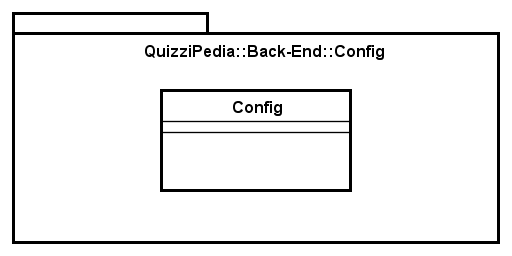
\includegraphics[scale=0.7]{UML/Package/QuizziPedia_Back-End_Config.png}
	\caption{QuizziPedia::Back-End::Config}
\end{figure}
\FloatBarrier

	\begin{itemize}
		\item \textbf{Descrizione}:
		\textit{package\ped{G}} contenente le componenti di configurazione del \textit{server\ped{G}};
		\item \textbf{Padre}: \texttt{Back-End};
		\item \textbf{Interazioni con altri componenti}:
			\begin{itemize}
				\item \texttt{App}:
				\textit{package\ped{G}} contenente le componenti del \textit{server\ped{G}} che implementano il \textit{pattern MVC\ped{G}}.
			\end{itemize}
		\item \textbf{Classi contenute}:
		\begin{itemize}
			\item \texttt{Config}: questa classe gestisce la configurazione del \textit{server\ped{G}}. \textit{Non sono stati modellati attributi e metodi di questa classe in quanto viene gestita da Express\ped{G}};
		\end{itemize}
	\end{itemize}

